Ir\documentclass{article}
% Language setting
% Replace `english' with e.g. `spanish' to change the document language
\usepackage[english]{babel}

% Set page size and margins
% Replace `letterpaper' with `a4paper' for UK/EU standard size
\usepackage[letterpaper,top=2cm,bottom=2cm,left=3cm,right=3cm,marginparwidth=1.75cm]{geometry}

% Useful packages
\usepackage{amsmath}
\usepackage{graphicx}
\usepackage[colorlinks=true, allcolors=blue]{hyperref}
\usepackage{chemmacros}
\usepackage{titlesec}
\titleformat*{\subsection}{\normalfont}
\usepackage{graphicx}
\graphicspath{ {./images/} }
\usepackage{array}
\usepackage{overpic}
\usepackage{tabularx}
\usepackage{multirow}
\usepackage{verbatim} % multi line comment pkg
\usepackage{algpseudocode}
\usepackage{cases}
\newcolumntype{L}{>{\RaggedRight\hspace{0pt}}X} 
\usepackage{subfig}
\title{10240 Group assignment on \ch{H2O2} decomposition}
\author{Group 31\\
Malgorzata Adrianna Dybowska-s215163\\
Veronica Miscu- s215159\\
Valeria Bubuioc- s215242}
\begin{document}
\maketitle

\section*{Individual contribution}

\section{Experimental measurements of the activity for \ch{H2O2} decomposition}

\subsection{Determine the activity of the metals you tested from a plot of volume of oxygen
vs. time. These plots may show a slight curvature. What could be the reason
for a decreasing measured activity? What could be the reason for an increasing
measured activity?} \\
The picture below show the volume of oxygen vs. time plots for different catalysts.\\
\begin{center}
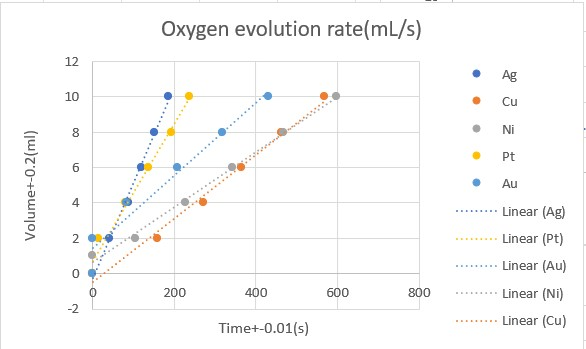
\includegraphics[width=\textwidth,height=\textheight,keepaspectratio]{oxygennnnn.jpg}
\caption{Pt/Ir}
\end{center}

 The catalitic activities are as follows:\\
 Ag-0.0108(mol/s/$m^2$) \\
 Au-0.0030(mol/s/$m^2$) \\
 Ni-0.0027(mol/s/$m^2$) \\
 Pt-0.0062(mol/s/$m^2$) \\
 Cu-0.0028(mol/s/$m^2$) \\


The reason for increasing measured activity could be due to 
Some of the reasons could be, (a) decomposition of the catalyst (sulphonic acid catalysts), (b) presence of polymeric material formed as by-product (for example, in case of trans-esterification of acrylic acid esters), which can camouflage the catalyst  (c) relatively large amount of residue formation, that can effectively reduce the catalyst concentration in the reaction mixture. (1) From this information we can deduce that its not (a) since we do not have sulphonic catalyst, and it is not (b) because it is we do not have polymeric materials. So we can conclude that the reason for decreasing in the measured activity is due to large amounts of residue formation, that can effectively reduce the catalyst concentration in the reaction mixture.


The reason for the 

\subsection{For the data from one metal wire, show how you quantified the uncertainty on
this specific activity measurement. (Hint: consider error propagation here)}

\subsection{For each metal you considered, submit the activity on this google form, to
share it with the rest of the class. The class’ responses are shown here.}

\section{Scanning Electron Microscopy Experiments}

\subsection{Determine the diameter of the Ir, Au, Rh, Pd, Ag, and Pt/Ir wires.}
\begin{center}
\begin{tabular}{ |c|c|c| } 
 \hline
 metal & name & diameter \\
\hline
 Ir & Iridium & 212 $\mu$m  \\
 Au & Gold &495 $\mu$m \\
 Rh & Rhodium & 499 $\mu$m  \\
 Pd & Palladium & 509 $\mu$m\\
 Ag & Silver & 989 $\mu$m\\
 Pt/Ir & Platinum/Iridium & 242 $\mu$m\\
 \hline 
\end{tabular}
\end{center}

\subsection{Include an image of the surface topography of the unused metal catalysts at
different magnifications. Consider which signal (SE or BSE), acceleration
voltage, and probe current to use.}
The following pictures in the next two tables were taken by the group number 2, because we did not manage to obtain good pictures with different magnifications.
\begin{center}
\begin{longtable}
\label{tab:long} \\
  \centering
  \begin{tabular}{ | m{7cm} | m{7cm} | }
    \hline
    Image & Catalyst details  \\ \hline
    \begin{minipage}{.3\textwidth}
      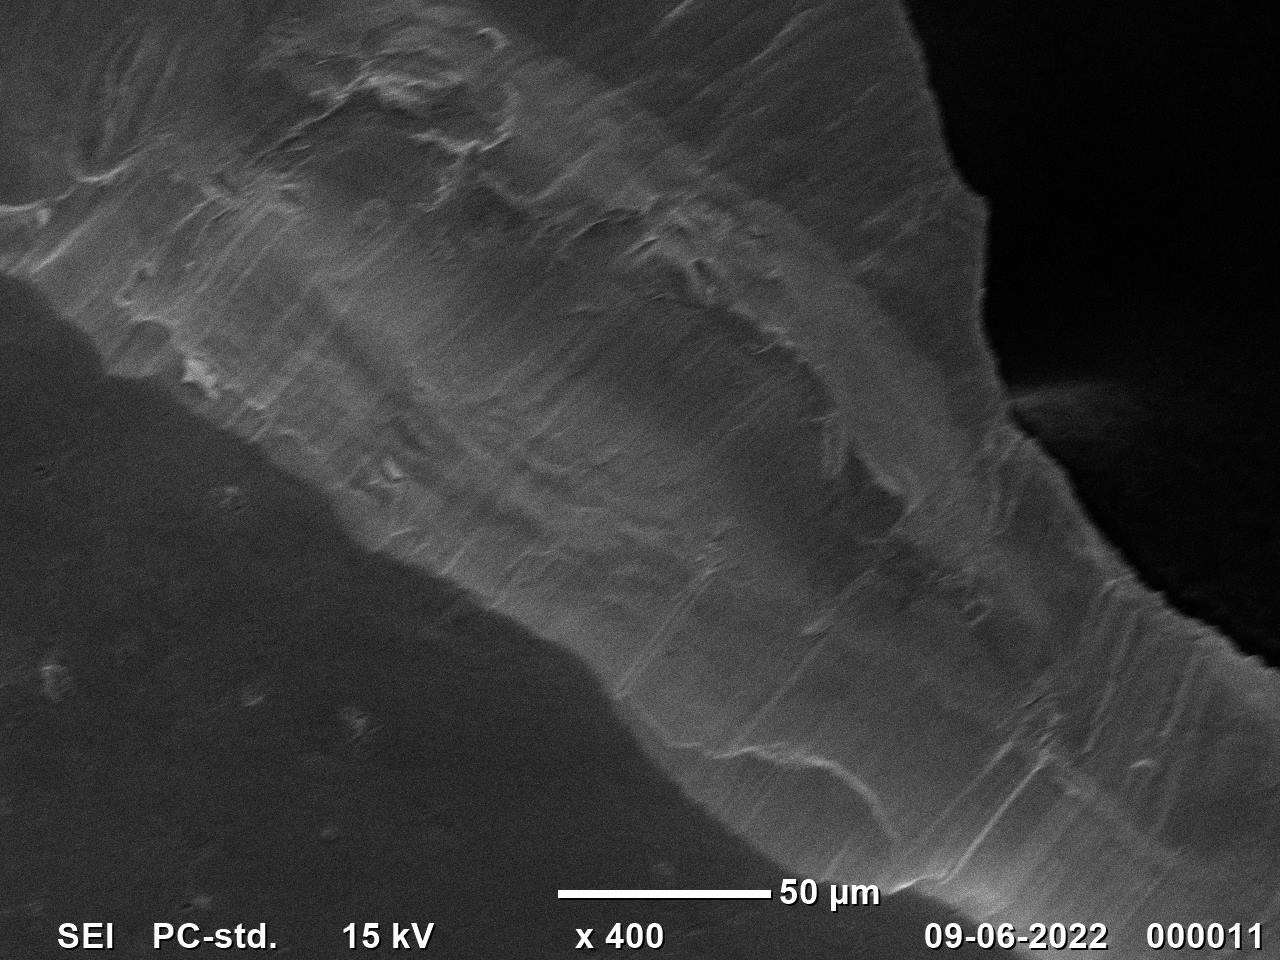
\includegraphics[width=60mm, height=60mm]{pictures/cu1.jpg}
    \end{minipage}
    &
    %\begin{minipage}[t]{5cm}
      \begin{itemize}
        \item unused Cu (copper)
        \item Magnification x400
        \item Acceleration voltage 15 kV
        \item Probe PC-std 
        \item Signal SEI 
      \end{itemize} \\ \hline
      \\
    %\end{minipage}
    \begin{minipage}{.3\textwidth}
      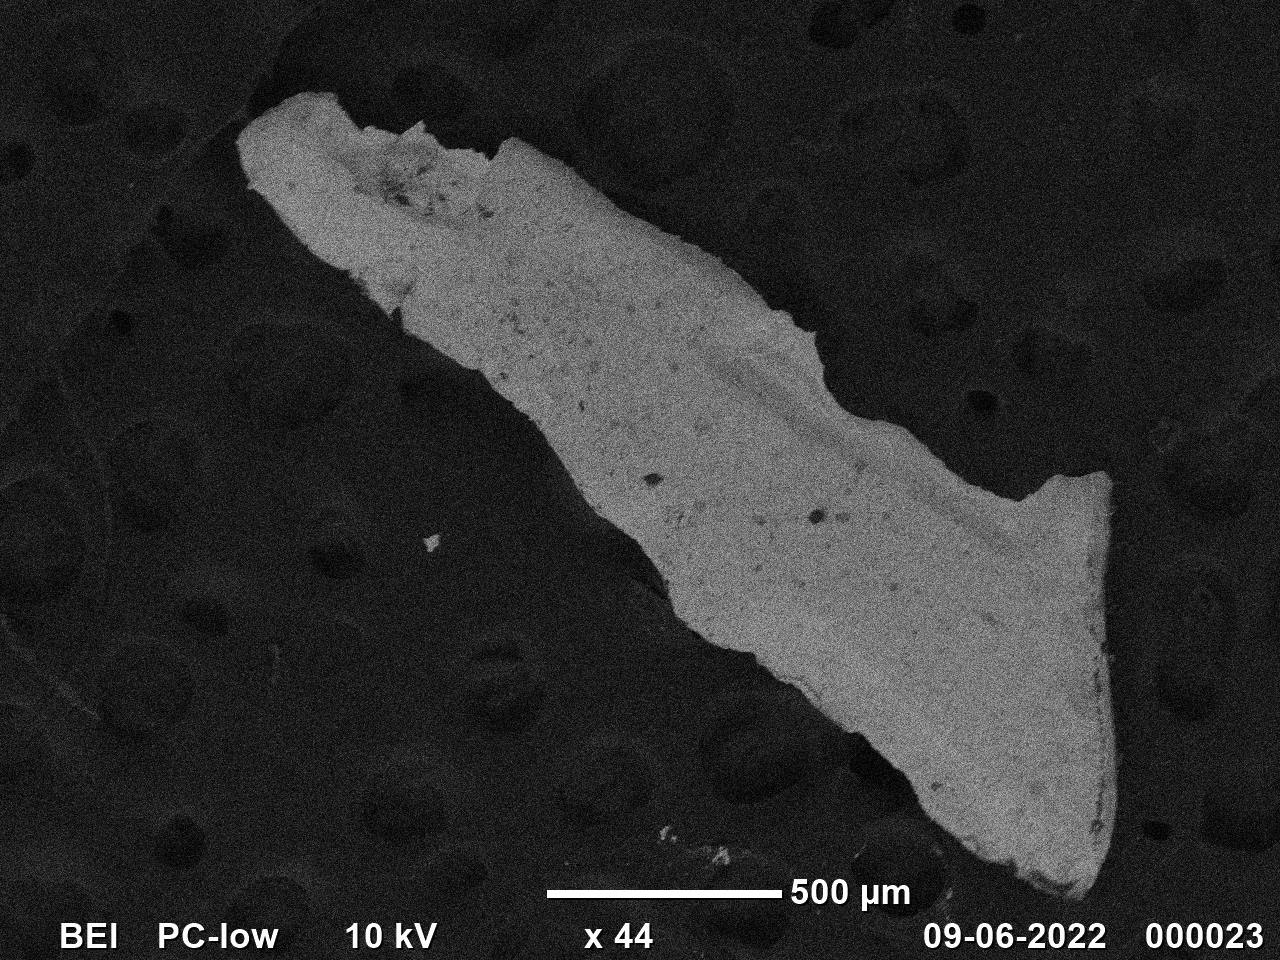
\includegraphics[width=60mm, height=60mm]{pictures/cu2.jpg}
    \end{minipage}
    &
    %\begin{minipage}[t]{5cm}
      \begin{itemize}
        \item unused Cu (copper)
        \item Magnification x44
        \item Acceleration voltage 10kV
        \item Probe PC-low
        \item Signal BEI
      \end{itemize} \\ \hline
    %\end{minipage}
    \\
    Continue on the next page & \\ \hline
    \end{tabular}
    \end{longtable}
\begin{longtable}   
\label{tab:long} \\
  \centering
  \begin{tabular}{ | m{7cm} | m{7cm} | }
    \hline
    Image & Catalyst details  \\ \hline
    \begin{minipage}{.3\textwidth}
      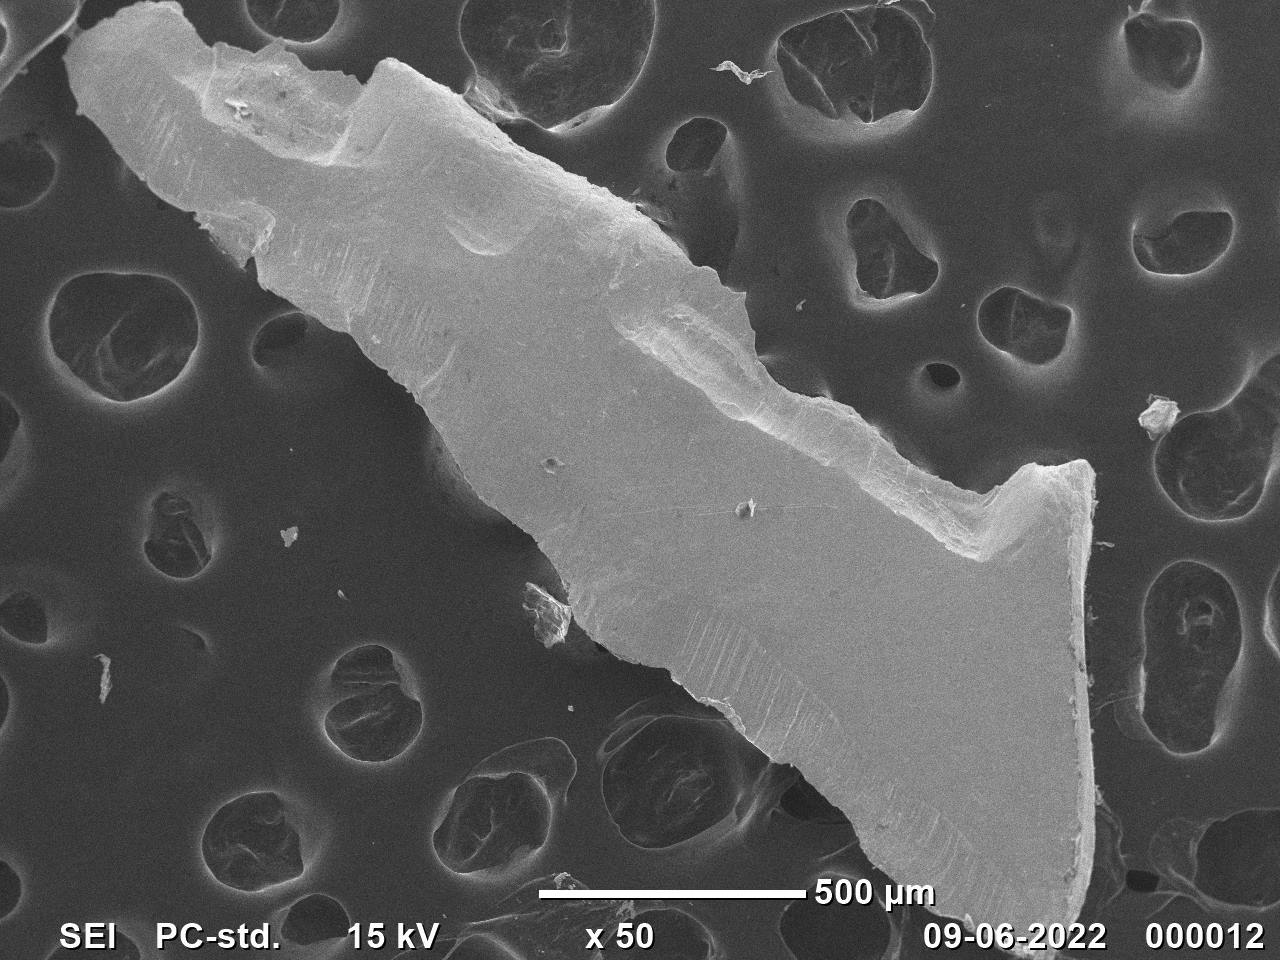
\includegraphics[width=60mm, height=60mm]{pictures/cu3.jpg}
    \end{minipage}
    &
    %\begin{minipage}[t]{5cm}
      \begin{itemize}
        \item used Cu (copper)
        \item Magnification x50
        \item Acceleration voltage 15 kV
        \item Probe PC-std
        \item Signal SEI
      \end{itemize} \\ \hline
      \\
    %\end{minipage}
    \begin{minipage}{.3\textwidth}
      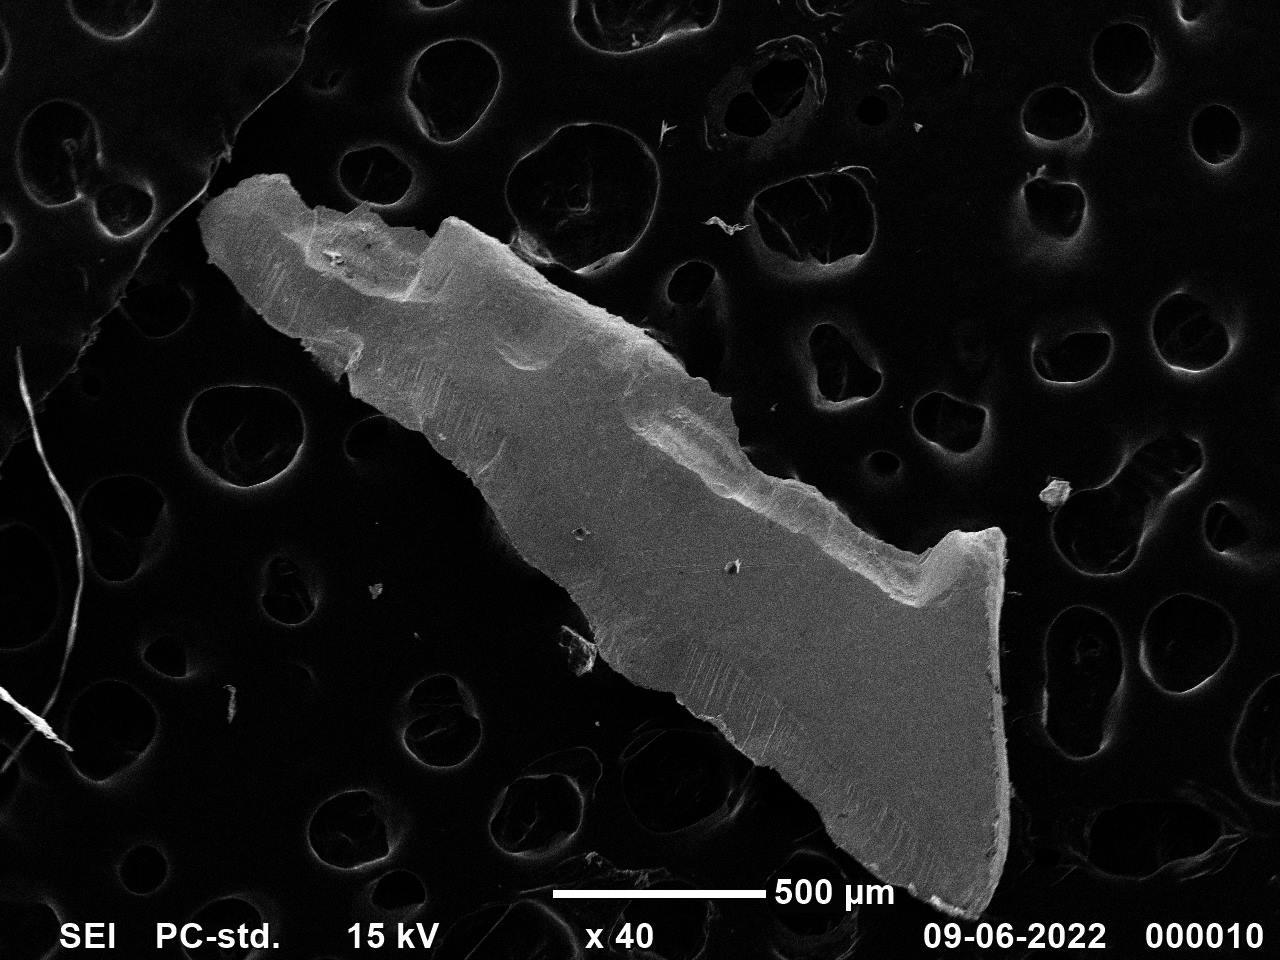
\includegraphics[width=60mm, height=60mm]{pictures/cu4.jpg}
    \end{minipage}
    &
    %\begin{minipage}[t]{5cm}
      \begin{itemize}
        \item unused Cu (copper)
        \item Magnification x40
        \item Acceleration voltage 15 kV
        \item Probe PC-std 
        \item Signal SEI 
      \end{itemize} \\ \hline
      \\
    %\end{minipage}
    \begin{minipage}{.3\textwidth}
      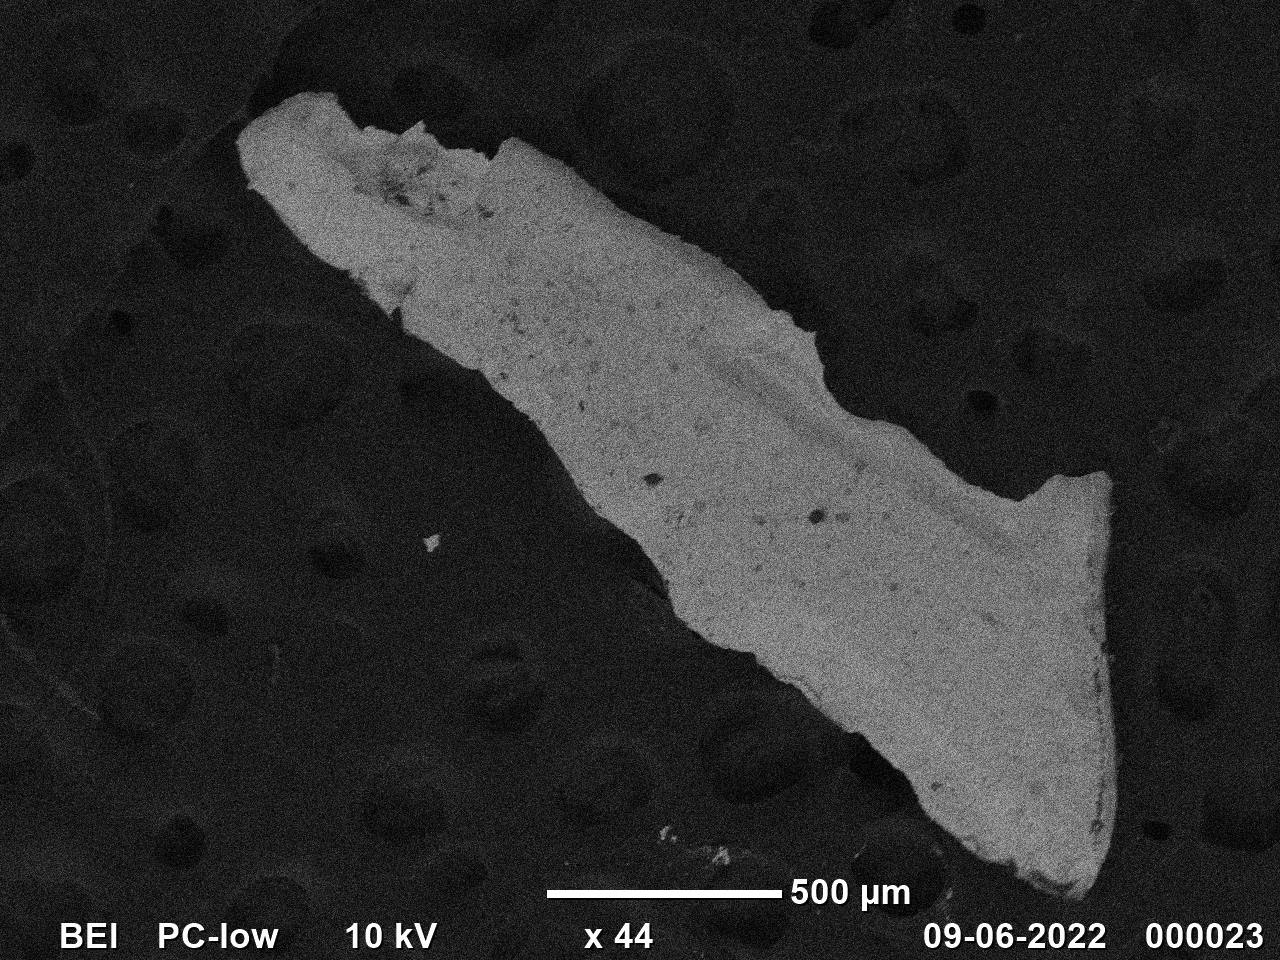
\includegraphics[width=60mm, height=60mm]{pictures/cu5.jpg}
    \end{minipage}
    &
    %\begin{minipage}[t]{5cm}
      \begin{itemize}
        \item unused Cu (copper)
        \item Magnification x44
        \item Acceleration voltage 10 kV
        \item Probe PC-low
        \item Signal BEI
      \end{itemize} \\ \hline
    %\end{minipage}
      \end{tabular}
\end{longtable}
\end{center}

\begin{longtable}
\label{tab:long} \\
  \centering
  \begin{tabular}{ | m{7cm} | m{7cm} | }
    \hline
    Image & Catalyst details  \\ \hline
    \begin{minipage}{.3\textwidth}
      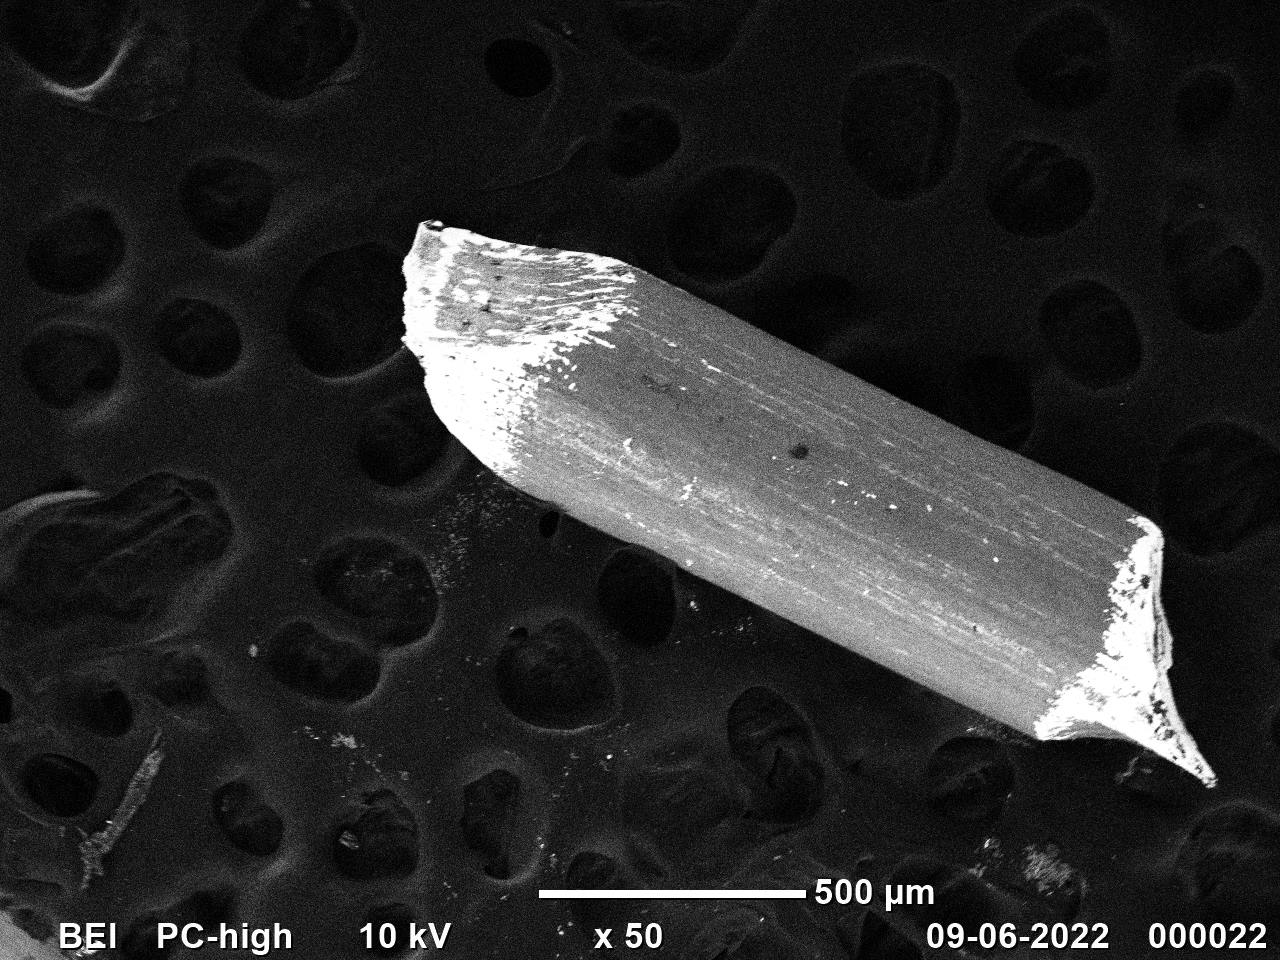
\includegraphics[width=60mm, height=60mm]{pictures/ptir1.jpg}
    \end{minipage}
    &
    %\begin{minipage}[t]{5cm}
      \begin{itemize}
        \item unused Pt/Ir (Platinum/Iridium)
        \item Magnification x50
        \item Acceleration voltage 10 kV
        \item Probe PC-high
        \item Signal BEI
      \end{itemize} \\ \hline
      \\
    %\end{minipage}
    \begin{minipage}{.3\textwidth}
      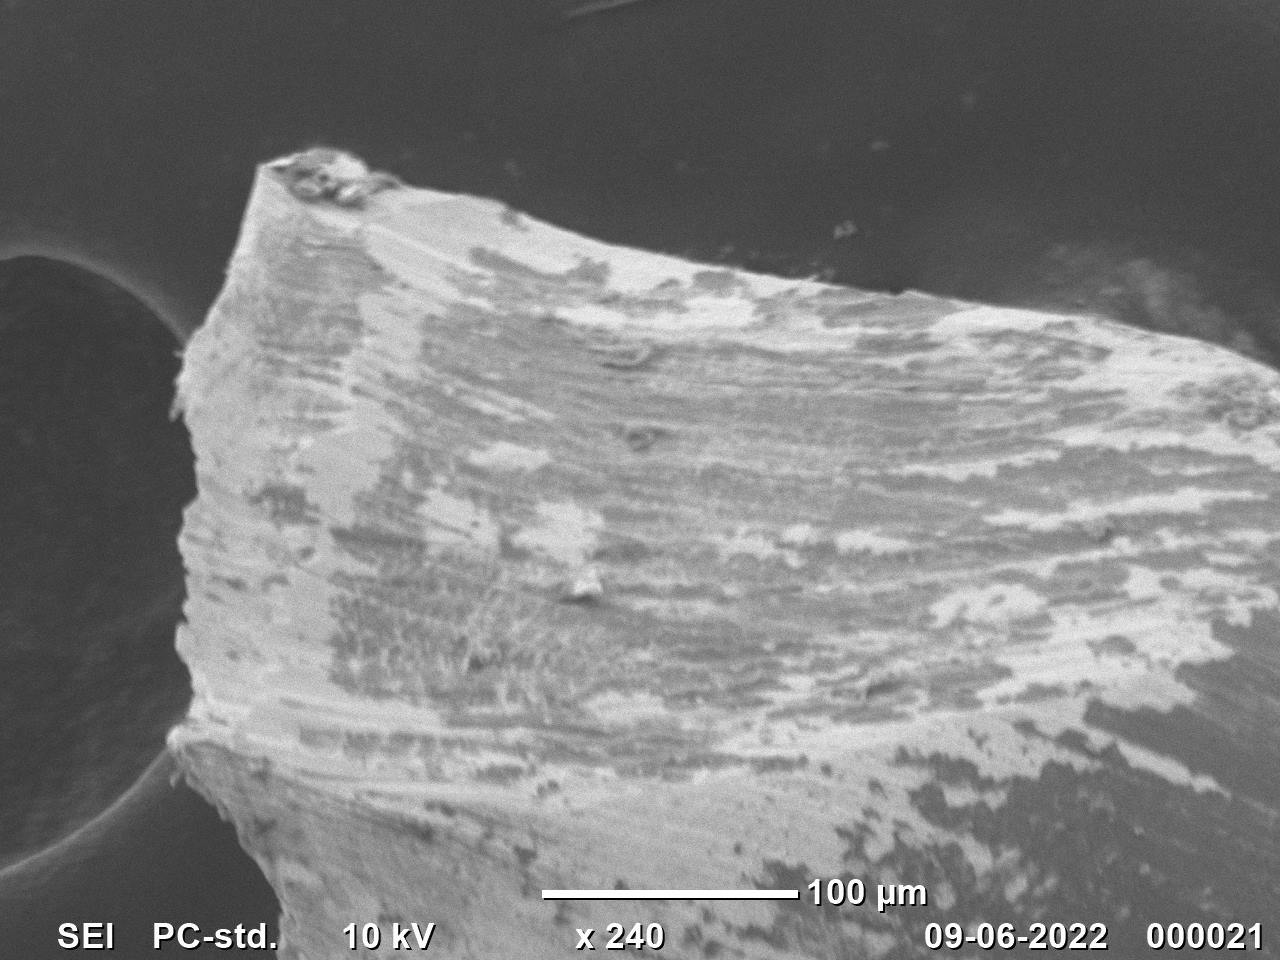
\includegraphics[width=60mm, height=60mm]{pictures/ptir2.jpg}
    \end{minipage}
    &
    %\begin{minipage}[t]{5cm}
      \begin{itemize}
        \item unused Pt/Ir (Platinum/Iridium)
        \item Magnification x240
        \item Acceleration voltage 10kV
        \item Probe PC-std
        \item Signal SEI
      \end{itemize} \\ \hline
    %\end{minipage}
    \begin{minipage}{.3\textwidth}
      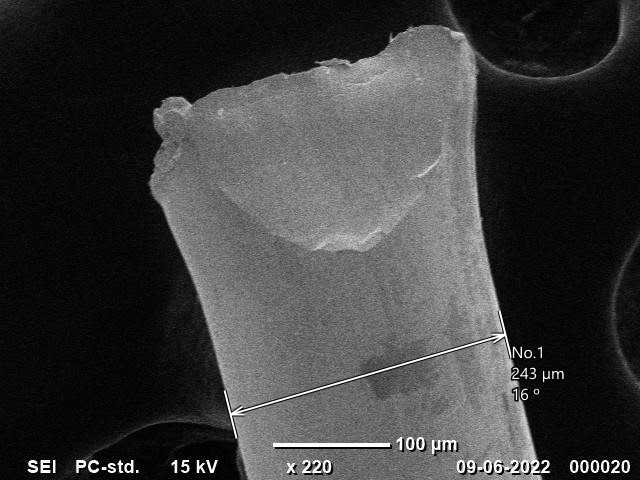
\includegraphics[width=60mm, height=60mm]{pictures/ptir3.jpg}
    \end{minipage}
    &
    %\begin{minipage}[t]{5cm}
      \begin{itemize}
        \item unused Cu (copper)
        \item Magnification x220
        \item Acceleration voltage 15 kV
        \item Probe PC-std
        \item Signal SEI
      \end{itemize} \\ \hline
    %\end{minipage}
 \end{tabular}
    \end{longtable}
\\
\begin{center}
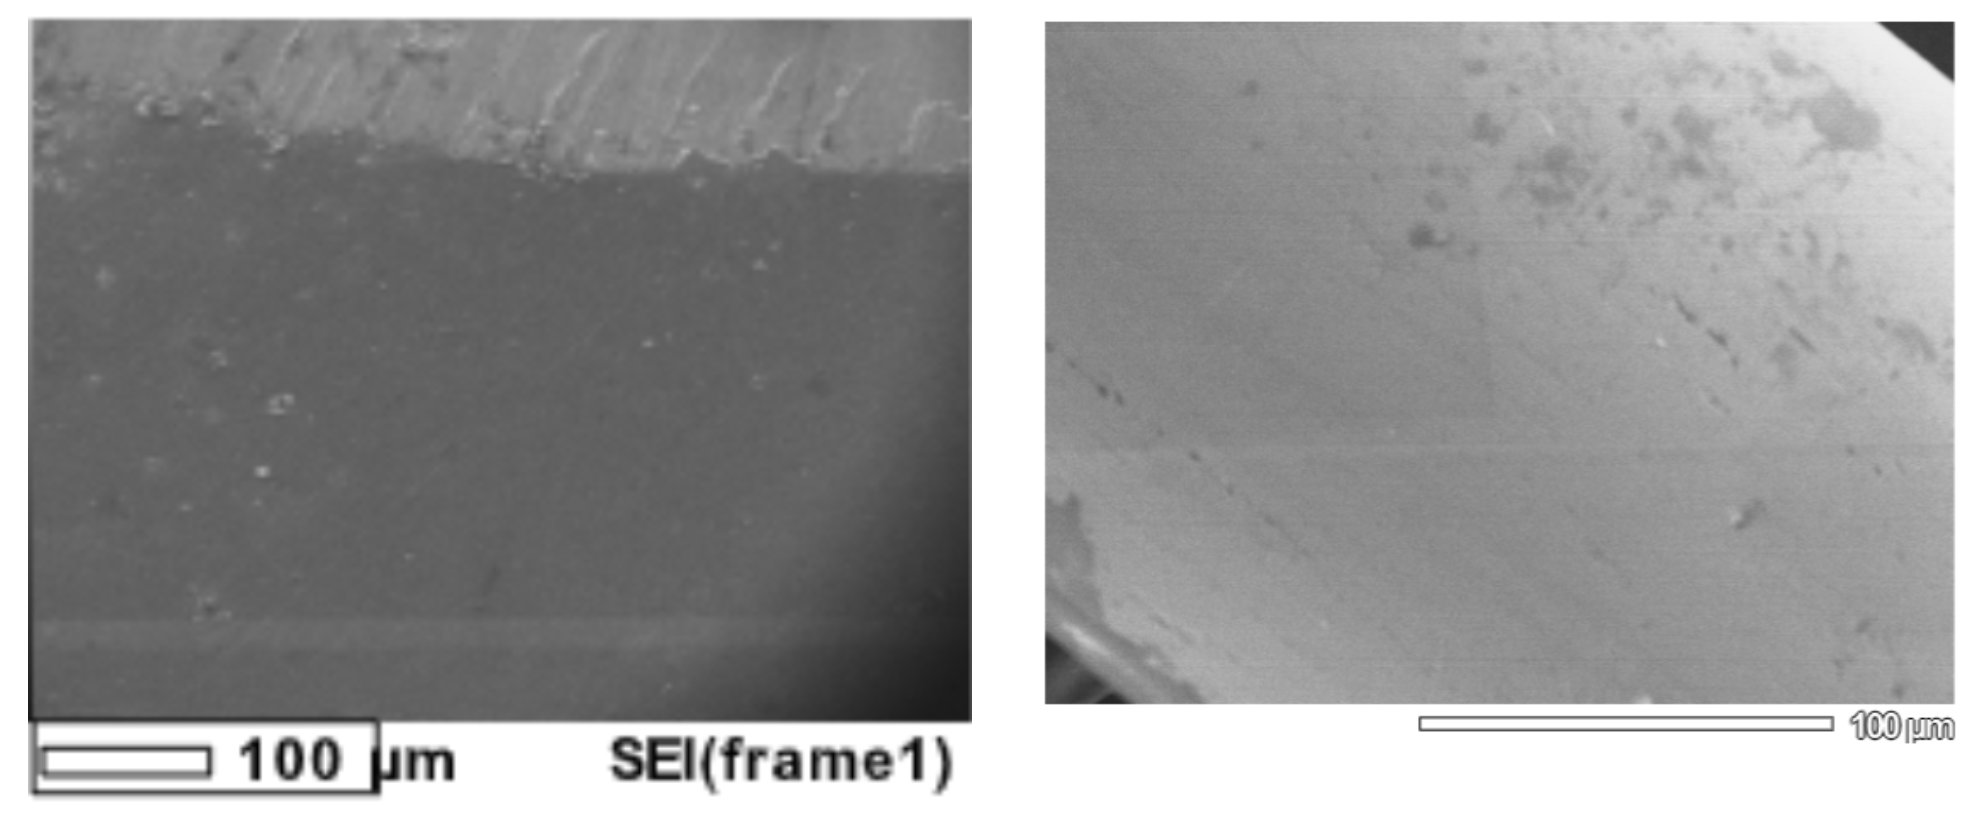
\includegraphics[width=\textwidth,height=\textheight,keepaspectratio]{pictures/CU and PT.png}
\caption{Unused Cu and Pt/Ir}
\end{center}

Our group used the acceleration voltage of 15kV and probe current- high(1 nA), as the images would be the most clear with such variables. For unused Cu we used SE as Cu was a piece of foil  and there wasn’t much difference in depth when we tried SE and BSE, and SE seemed more clear. For unused Ir/Pt we used BSE, to get more of a 3D visualization, however since it is unused it wasn’t as visibly porous. 

\subsection{Determine the chemical composition of the Cu foil and Pt/Ir wire using EDS.}

For Pt/Ir:
Oxygen could be due to oxidation.
Carbon could be from the carbon tape under the specimen. 

\begin{center}
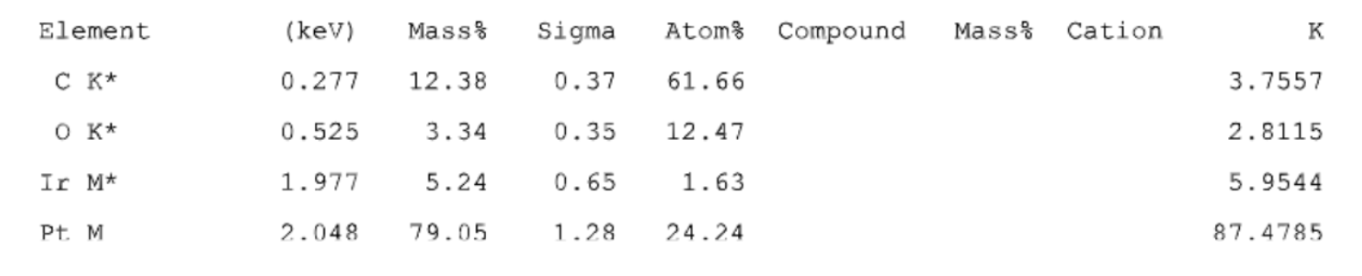
\includegraphics[width=\textwidth,height=\textheight,keepaspectratio]{pictures/ptir.png}
\caption{Pt/Ir}
\end{center}
For Cu foil:
Oxygen could be due to oxidation.
Carbon could be from the carbon tape under the specimen. 

\begin{center}
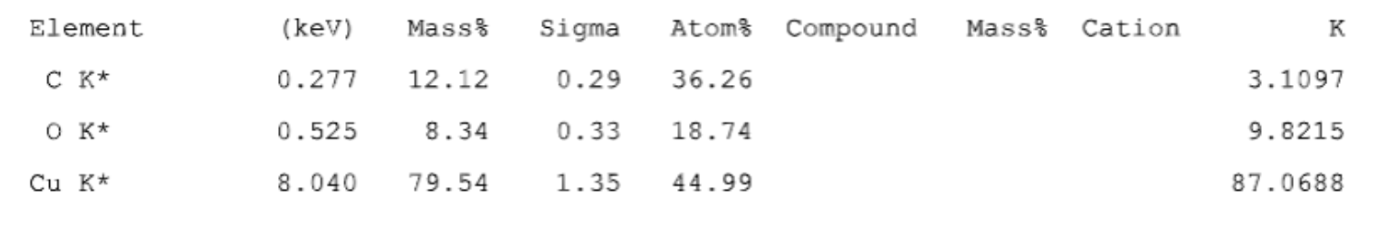
\includegraphics[width=\textwidth,height=\textheight,keepaspectratio]{CUfoil.png}
\caption{Cu foil}
\end{center}
\subsection{Determine any chemical and structural changes for the Cu and Pt/Ir catalysts
on unused and used samples.}

Used copper had traces of silver. It also had a higher concentration of carbon. Smaller concentration of oxygen. Traces of fluorine. \\

Used Platonium/Iridium has traces of silver. More oxygen and more carbon. \\


\section{Xray Diffraction/Absorption Spectroscopy Experiments}

\subsection{Plot the intensity as a function of energy for the measurements you made
without filters with energy E in eV by using eq. (5) in your lab manual. Explain
the shape of this curve – e.g. does the maximum energy which you see in the
brems spectrum \match the accelerating voltage you have used? Identify as
many of the characteristic lines as you can.}
\begin{center}
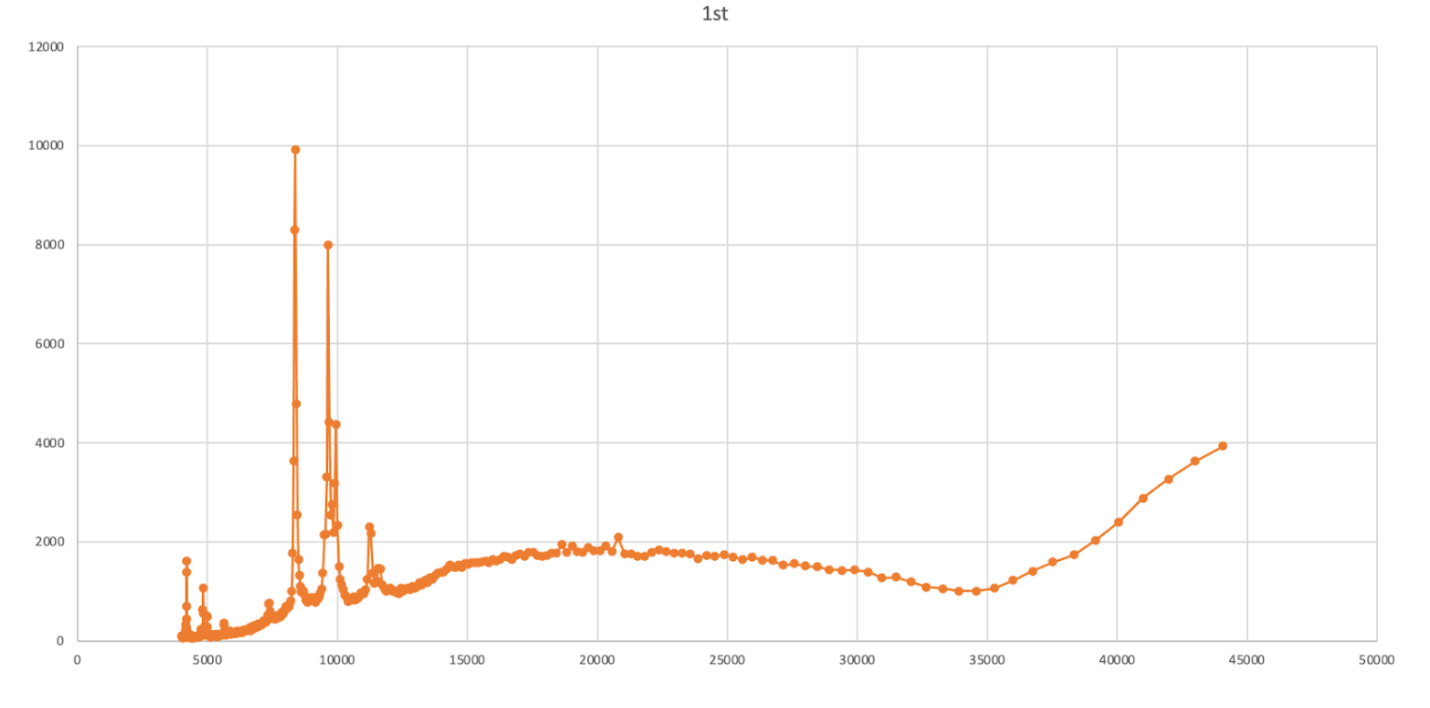
\includegraphics[width=\textwidth,height=\textheight,keepaspectratio]{pictures/3a.png}
\caption{Pt/Ir}
\end{center}

\begin{center}
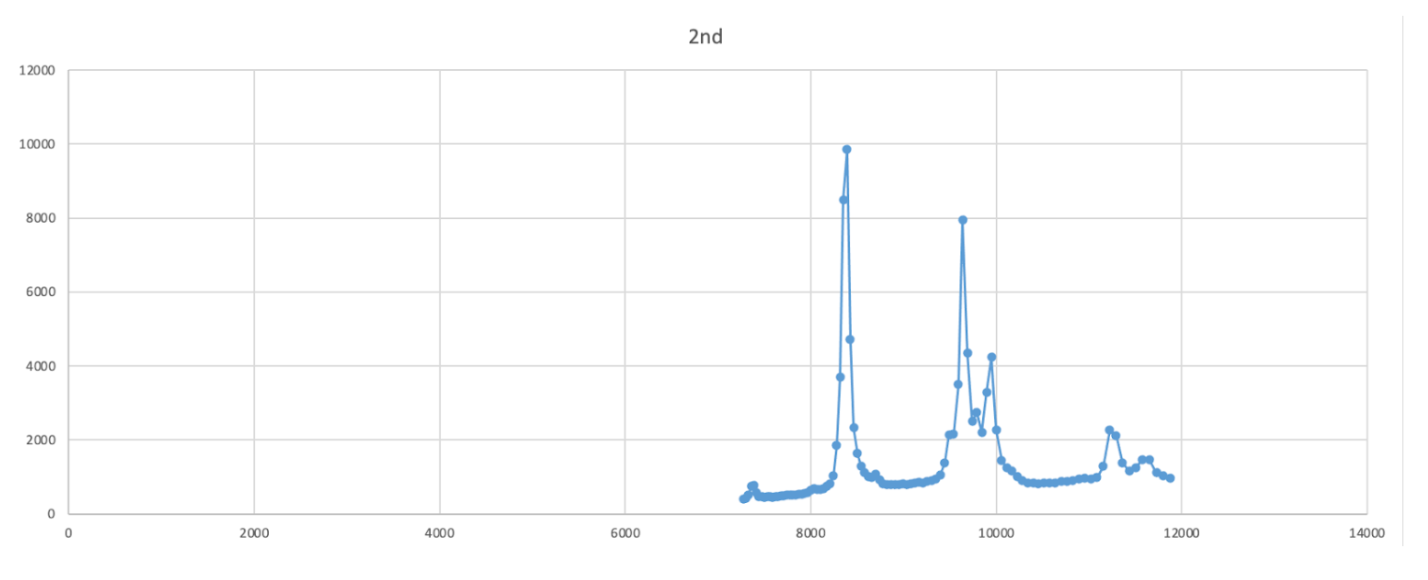
\includegraphics[width=\textwidth,height=\textheight,keepaspectratio]{pictures/3aa.png}
\caption{Pt/Ir}
\end{center}

The peaks seen on the graphs are related to the braking acceleration and their magnitude depends on the anode material on the x-axis. Other observations we made:

\begin{itemize}
  \item small angle = high energy,  big angle = low energy;
  \item positions of characteristic lines DO NOT depend on the acceleration voltage, Ua;
  \item does not make sense to get higher than 35kV, because acceleration voltage setted is 35 kV.
\end{itemize}

\subsection{Plot the intensity as a function of energy for the measurements you have
made with the thin filters (Ni, Cu and Zn 0.025 mm). Plot the measurement
you made without filter in the same graph. Comment on interesting
differences and similarities between the measurements.}



\begin{center}
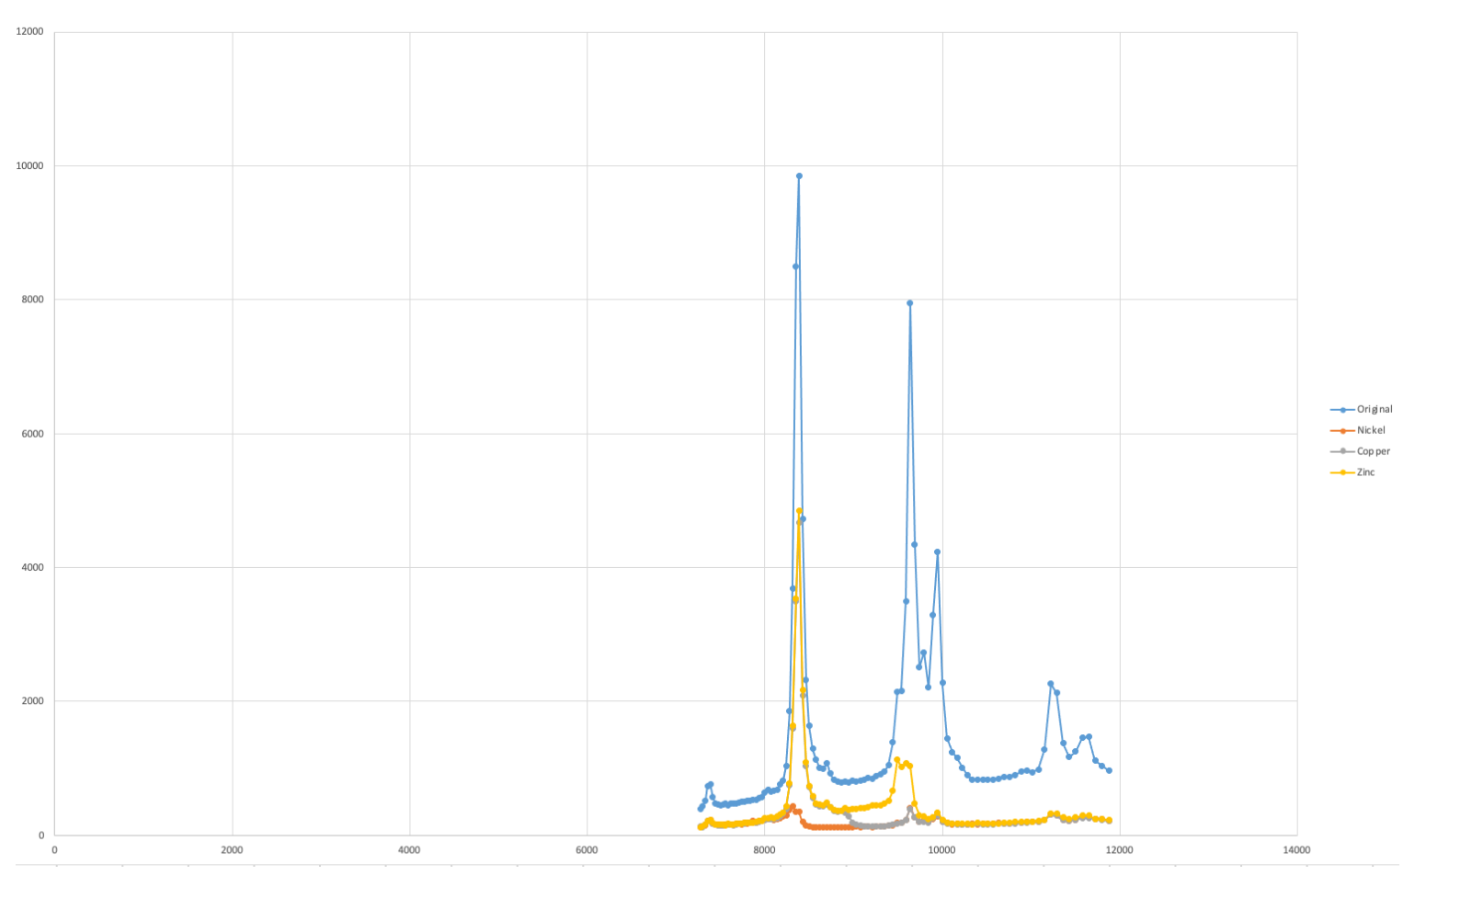
\includegraphics[width=\textwidth,height=\textheight,keepaspectratio]{pictures/3b.png}
\caption{Pt/Ir}
\end{center}

The very first thing that can be seen from the graph is obviously the differences in intensity profiles. We can see the Nickel has the same intensity as the anode, so the x-ray kicks out the electron in Nickel. On the other hand, there is not enough energy to do the same with Zinc and Copper, so it goes right through.

\subsection{Plot the intensity as a function of energy for the spectra you made with the
thin filters (Ni, Cu and Zn 0.025 mm) divided by the measurement you made
3
without filter. Then calculate and plot the transmittance: INi/I0, ICu/I0 and
IZn/I0 together in a new graph. Include your table from the lab manual
question 7.4 and comment on possible trends and discrepancies in the
results.}
\begin{center}
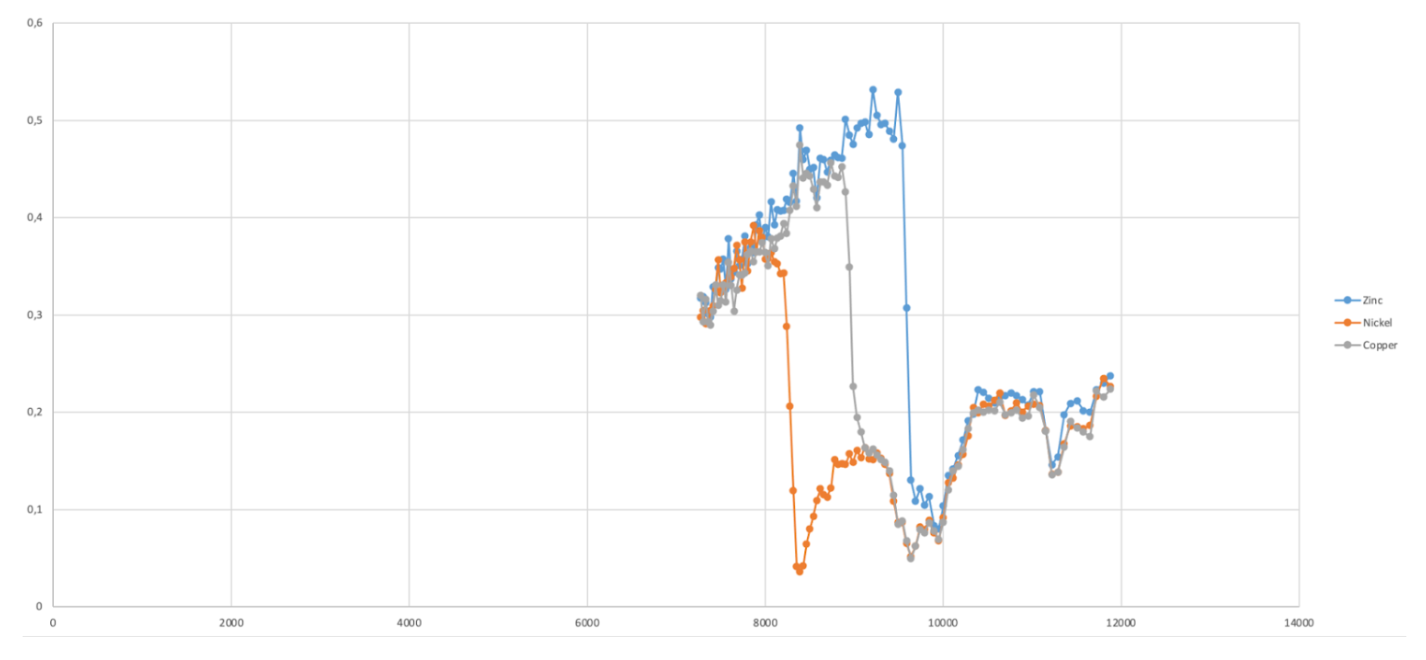
\includegraphics[width=\textwidth,height=\textheight,keepaspectratio]{pictures/3c.png}
\caption{Pt/Ir}
\end{center}
What can be deduced from this part is that Zn needs the most energy from X-ray to kick out electrons, which results in higher transmittance. Nickel has the second highest transmittance and copper has the lowest one. This corresponds to the statement we saw in the theory part: “the energy of the characteristic peaks will depend on the anode material and will generally be higher for materials with a higher atomic number”: Zn has the atomic number 30, Nickel is 29 and Copper is 28.

\section{Review of catalysts and the energy landscape of a reaction}

\subsection{Consider the following potential energy landscape for a generic reaction. Mark
on the plot the reaction energy, $ \Delta G$, and also the activation energy, $G_a$}
\begin{center}
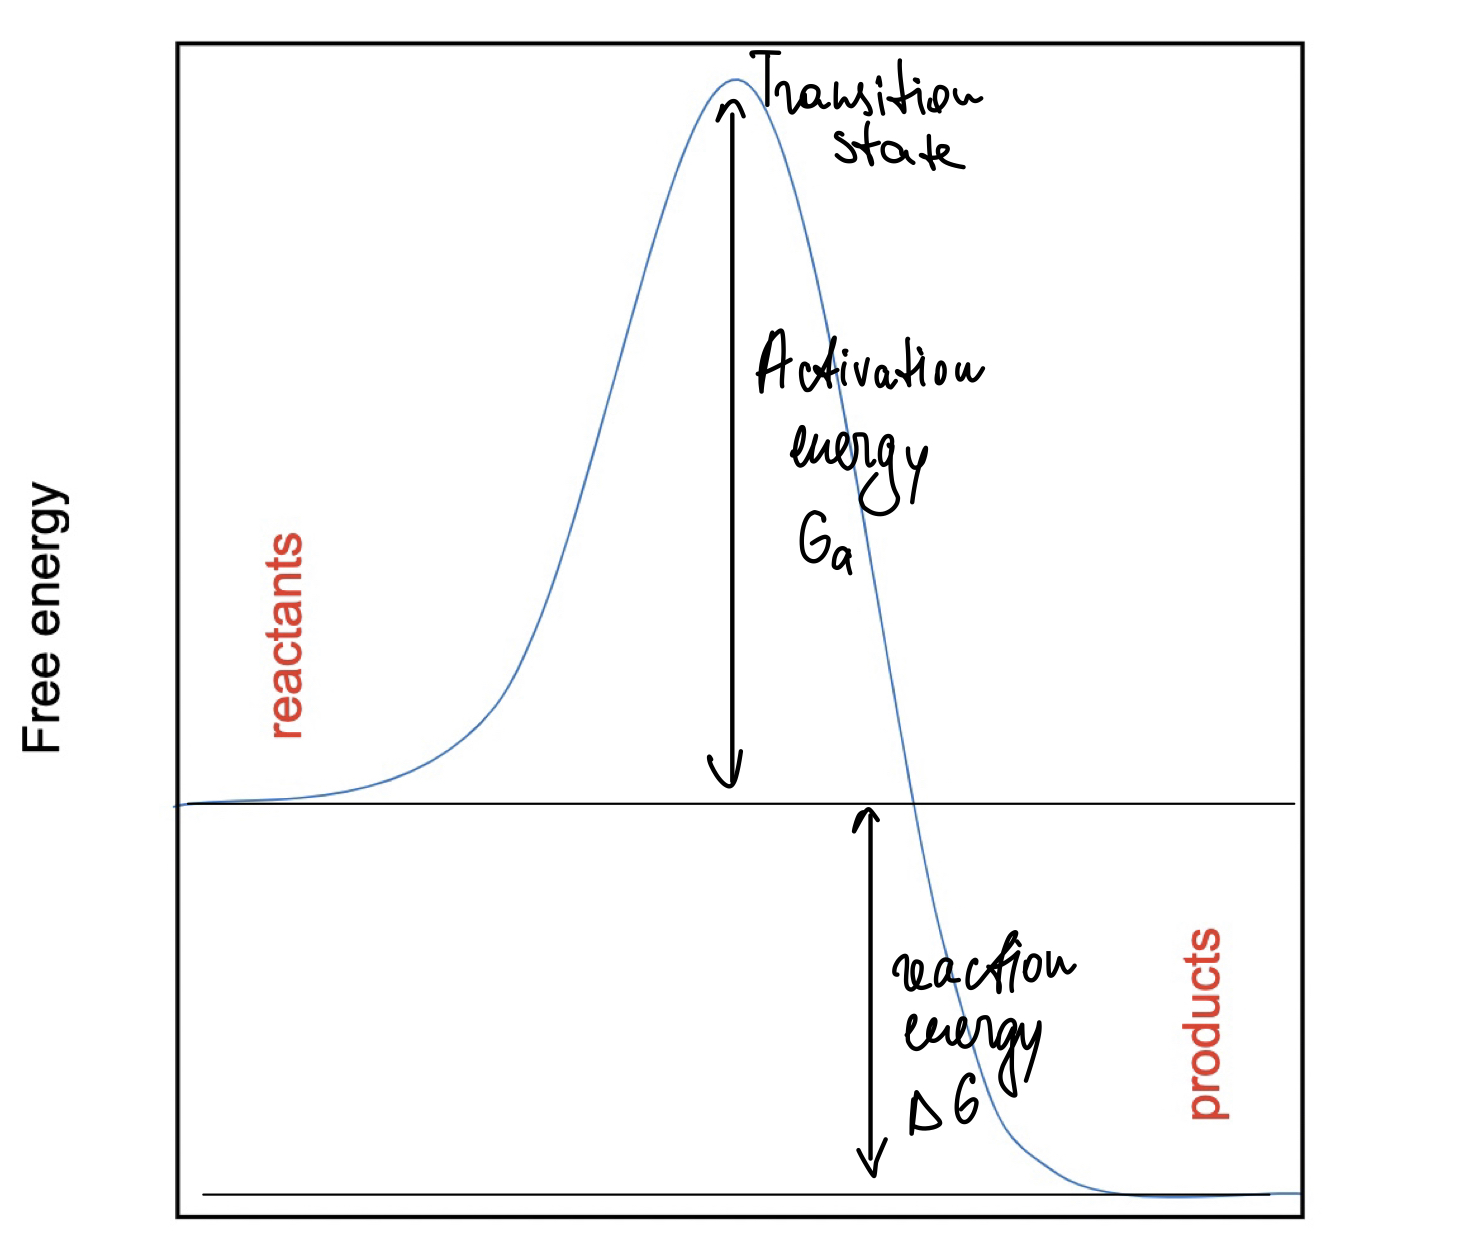
\includegraphics[width=\textwidth,height=\textheight,keepaspectratio]{pictures/4a.jpeg}

\end{center}
\subsection{Now imagine that the reaction takes place in the presence of a catalyst, which
speeds up the reaction rate. Draw how the potential energy diagram might
change in this case.}
\begin{center}
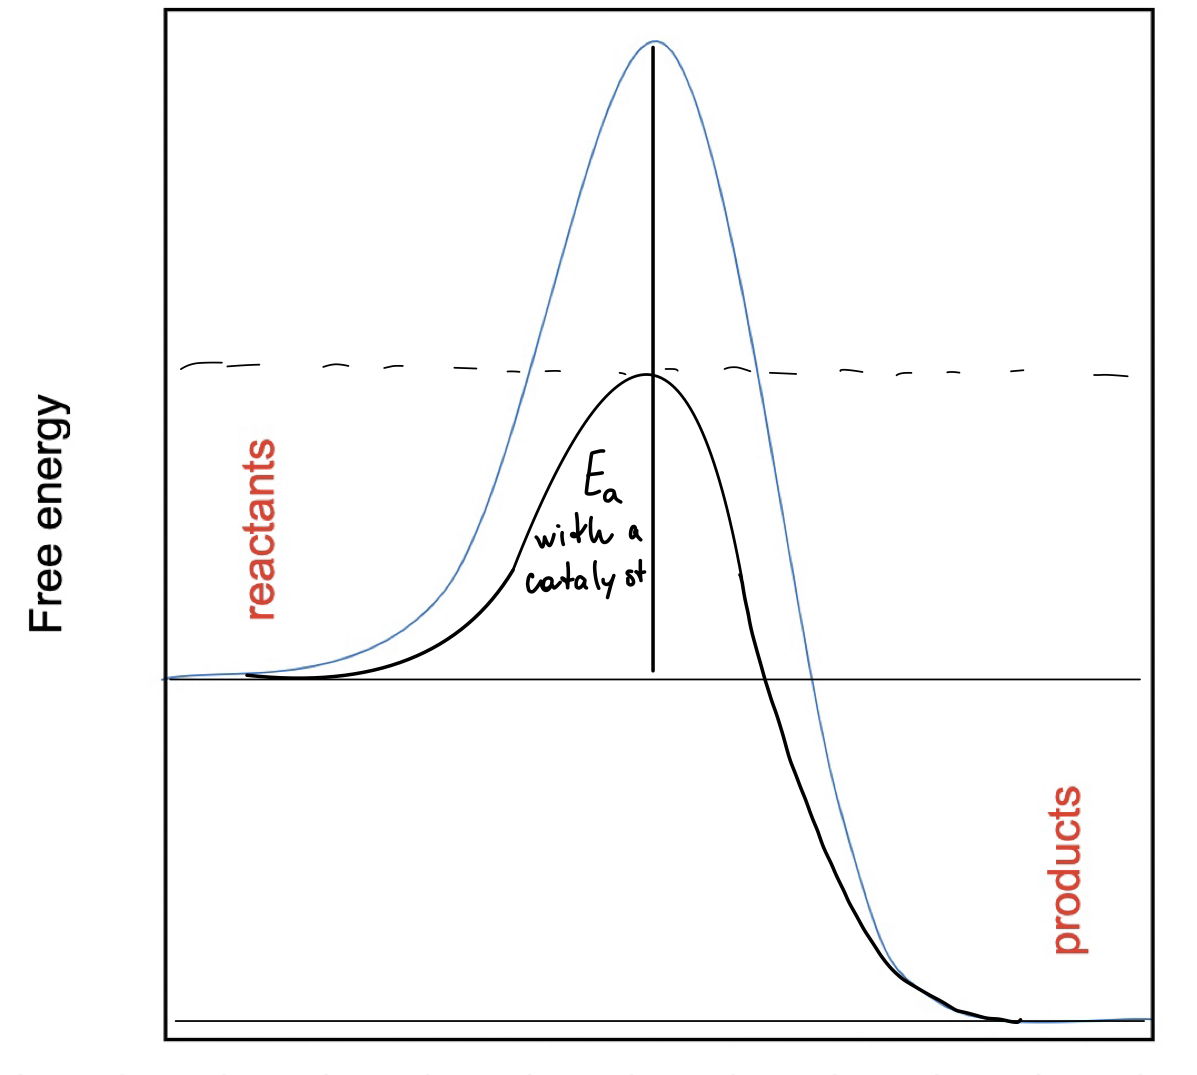
\includegraphics[width=\textwidth,height=\textheight,keepaspectratio]{pictures/4b.jpeg}

\end{center}
\\
\section{\ch{H2O2} decomposition mechanism}
\\
\subsection{\ch{H2O2(aq)} decomposes into \ch{H2O(l)} and \ch{O2(g)}. Write out the balanced overall
reaction.}
\\ 2\ch{H2O2}_{(aq)} = 2\ch{H2O_{(l)}} + \ch{O2_{(g)}}
\\ \ch{H2O2}_{(aq)} = \ch{H2O_{(l)}} + \frac{1}{2}\ch{ O2_{(g)}}

\subsection{In the presence of a solid (heterogeneous) catalyst, \ch{H2O2(aq)} undergoes
dissociative adsorption and decomposes into 2 adsorbed OH species. A free
surface site is denoted by the symbol * and OH adsorbates by *OH. Let us
assume that this first step is slow and rate limiting for the overall reaction. Write
out the balanced chemical equation for this elementary step.}

\\ \ch{H2O2}_{(aq)} +2\ast =  2\ch{OH \ast}
\subsection{Let us assume that the remaining elementary steps are fast and not rate
limiting. While the specific steps are not known, if they are fast, we can assume
they are in equilibrium. Write out one single overall balanced chemical
equation for the sum of these remaining processes (not including the
elementary step you wrote in (b)).}

\\\ch{OH \ast} + \ch{H2O2}_{(aq)} = 2\ch{H2O_{(l)}} + 2\ast + \ch{O2_{(g)}}

\section{Scaling relations and the Sabatier principle}
\subsection{Collect the available activation and adsorption free energies for various metals
from electronic structure calculations. (see the “GBAR” manual uploaded on
LEARN for how to do so). We also provide the energies for the oxides below,
which you will include in your plot in b.}
\begin{center}
\begin{tabular}{ |c|c|c| } 
 \hline
 metal & activation free energy(eV) & adsorption free energy for OH(eV) \\
\hline
 Ag111 & 0.97 & 1.54 \\
 Au111 & 1.33 & 1.72 \\
 Cu111 & 0.82 & 1.11 \\
 Ir111 & 0.68 & 1.38\\
 Pd111 & 0.83 & 1.58\\
 Pt111 & 0.99 & 1.30\\
 Rh111 & 0.75 & 1.41\\
 \hline 
\end{tabular}
\end{center}
\subsection{Plot the activation energies $G_a$ vs. the OH adsorption energies $\Delta G(OH \ast )$ you have collected. What trend do you see? Why might there be such a trend?
Are there outliers? (Note that error bars for the computed energies are 0.1-
0.2eV.) Write an equation for the relationship between $G_a$ and $\Delta G(OH \ast)$. Use
this equation to fit a curve through the points on the plot, and we will use the
fitted parameters in question 7.
This type of scaling is in fact very general in heterogeneous catalysis. For the
metals, plot the adsorption energy of *O, $\Delta G(O \ast)$, vs. $\Delta G(OH \ast)$. Let us define
$\Delta G(O \ast)$ with the same references as we used for $\Delta G(OH \ast)$, as follows:}
$$\Delta G(O \ast)=G(O \ast)-G(\ast)-(G(\ch{H2O_(_l_)})-G(\ch{H2_(_g_)})) $$
These “scaling relationships” arise from the similarity between the interactions
of adsorbates and transition states with the electronic structure of the substrate.
As you will see, they are really helpful in rationalizing the trends in activity
amongst different catalysts. \\

\begin{center}
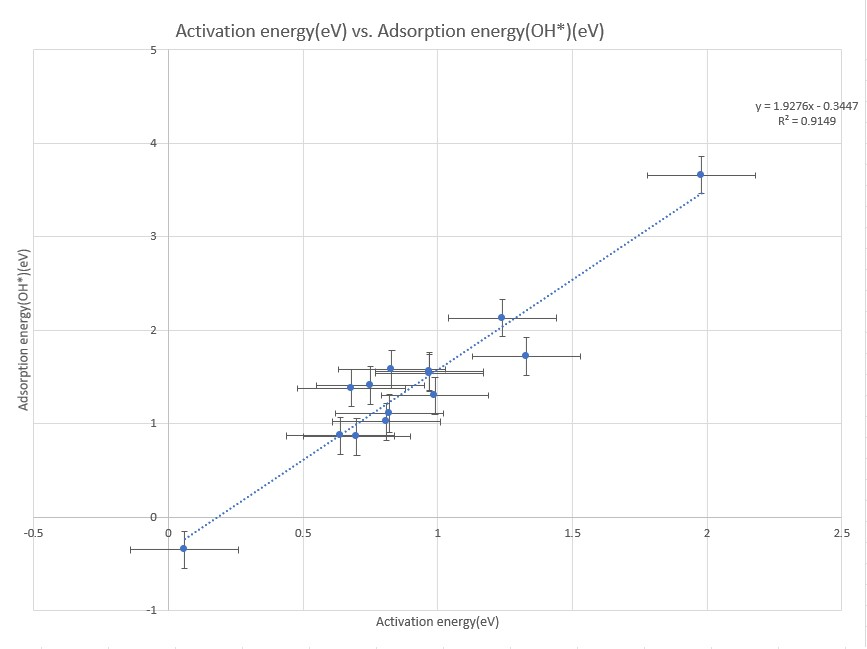
\includegraphics{6.2.a.jpg}
\caption{Activation energy vs. Absorption energy of OH}
\end{center}
 \\
The picture above presents the relationship between the activation free energy against the adsorption energy for OH*
There is a linear trend between the points on the plot. Au111 is the most visible outlier(error bars are 0.2eV) ,Pd111, Rh111, Ir111 are also outliers.
The equation for the relationship between activation free energy and adsorption energy for OH* is:\\
$y=1.9276x-0.3447$\\

\begin{center}
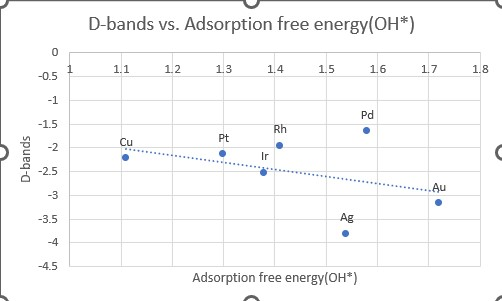
\includegraphics{pictures/6.2.b.jpg} \\
\caption{Absorption energy of $O\ast$ vs. Absorption energy of $OH\ast$}
\end{center}
 \\
The picture above presents the relationship between adsorption energies of O* for different metals against the adsorption energy for OH*. \\

\subsection{Determine the d-band centers for the bare slabs (as described in the GBAR
Guide). Plot $\Delta G(OH \ast)$ of the metals against the d-band centers you have
computed. What trend do you see? Are there outliers and why do you think
they might be present?}

\begin{center}
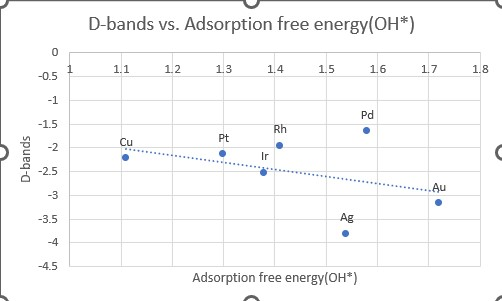
\includegraphics{pictures/6.3.jpg}
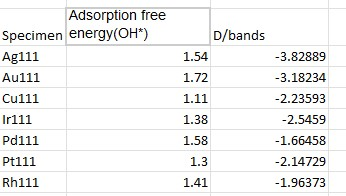
\includegraphics{data d.jpg}
\caption{Absorption free energy of $O\ast$ vs. D-bands data and plot}
\end{center}

 \\

The adsorption energy should increase across the periodic table, however in this plot it is not the case. It indeed starts with Cu at the lowest adsorption energy and Au at the highest, however the middle metals are mixed. 

The trend shows that the higher the adsorption energy the weaker the binding.The metals Cu, Ir and Au follow the trend well, however there are some outliers like: Pd, Ag, Rh, Pt. 

\section{Kinetic modelling}
\subsection{Consider the rate limiting (slow) step you wrote down in question 5b. Write out an expression for the forward rate \textbf{$r_1$} (assume the backward rate is negligible)
in terms of the coverage of free sites $\theta\ast$ and the concentration of hydrogen
peroxide, $c_\ch{H2O2}$. The corresponding proportionality constant, $k_1$, is the \textit{rate constant}, which is given by transition state theory as follows:
$$k_1=\frac{k_b*T}{h}*e^-^\frac{G_a}{k_B*T}$$
where $k_b$ is the Boltzmann constant, \textit{T} the temperature, and \textit{h} Planck’s
constant, and $G_a$ is the activation energy which you collected in Question 6a.}

\\r_{1} = C_{\ch{H2O2}\cdot \theta \ast}
\subsection{To determine \textbf{$r_1$} from the expression in question 7a, you need the coverage of free sites $\theta\ast$. $\theta\ast$ can be determined in terms of the equilibrium constant, K, and pressure of oxygen $p_\ch{O2}$ , $\theta\ast$ , and $\theta_\ch{OH}$ associated with the “fast” step you wrote down in question 5c. Write out the K for this “fast” step in terms of the
pressure of oxygen $p_\ch{O2}$ , $\theta\ast$ , and $\theta_\ch{OH}$).
Now, for surface reactions, the corresponding “concentration” of an adsorbed
species i is its surface coverage, $\theta_i$. For example, for a reaction $aA\ast + bB_(_g_) ⇄
cC_(_a_q_) + d\ast$, the equilibrium constant is $K=\frac{[C]^c*\theta^d_\ast}{\theta^a_A*p^b_B}$
Liquid and solid phases have fixed densities, and therefore do not need to be
included explicitly in K.}

\subsection{Now, assume that the only adsorbate on the surface with any significant
coverage is \ast OH. Using this assumption, and the expression for K in 7b, write
out an expression for the coverage of free sites $\theta_\ast$}

\subsection{}

\section{Understanding the shape of the activity curve}
\subsection{One way to understand the shape of the theoretical activity volcano plot from 7e is
to look at the different contributions to the overall rate:
\begin{enumerate}
    \item Plot the $k_1$ as a function of $\Delta G_O_H$ (you may wish to use a log scale on
the y-axis here, since exponential functions “blow up”)
    \item Plot $\thera\ast$, as a function of $\Delta G_O_H$
\end{enumerate}
What trends do you see in $k_1$ and $\thera\ast$ as $\Delta G_O_H$ increases (weak binding) or
decreases (strong binding)? Why is there an optimal activity at intermediate $\Delta G_O_H$
?}
\section{Comparison to experimental rates}
\subsection{From the experimental rates on metals determined by the class (as well as
those for the oxides, given to you in your lab manual), plot the average activities
for each metal, also normalized by the experimentally determined rate on Ag,
again as a function of $\Delta G\astOH$. Include error bars on the activities (recall:
standard deviations of the mean; here we are considering statistical
uncertainties on the class averages, vs. the error propagation you considered
in Question 1). For Pt/Ir, you have determined its composition in your EDS
measurement. Make a guess of its $\Delta G\astOH$ in the plot here, based on the Pt
and Ir $\Delta G\astOH$.
The reason we suggest to compare the normalized rate volcanoes is that
computations usually predict trends better than the actual rates, given the
uncertainties in the computed energies.}

\section{reference}
(1) https://www.researchgate.net/post/What-are-the-pssible-reasons-for-reduced-activity-selectivity-of-a-recovered-catalyst
\end{document}